\documentclass{article}

\usepackage{graphicx}
\graphicspath{ {./images/} }

\begin{document}
 \section{Problem 1}
\subsection{a}
Using the 2nd order upwind method, the following equations are constructed: \newline
$u>0 \> ; \> v>0$: \newline
\newline
$\frac{\phi^{n+1}_{i,j}-\phi^{n}_{i,j}}{\Delta t} = u_{i,j}\frac{-3\phi^{n}_{i,j} + 4\phi^n_{i-1,j} - \phi^{n}_{i-2,j}}{2\Delta x} + v_{i,j}\frac{-3\phi^{n}_{i,j} + 4\phi^n_{i,j-1} - \phi^{n}_{i,j-2}}{2\Delta y}$ \newline
\newline
\newline
$u<0 \> ; \> v>0$: \newline
\newline
$\frac{\phi^{n+1}_{i,j}-\phi^{n}_{i,j}}{\Delta t} = u_{i,j}\frac{3\phi^{n}_{i,j} - 4\phi^n_{i+1,j} + \phi^{n}_{i+2,j}}{2\Delta x} + v_{i,j}\frac{-3\phi^{n}_{i,j} + 4\phi^n_{i,j-1} - \phi^{n}_{i,j-2}}{2\Delta y}$ \newline
\newline
\newline
$u>0 \> ; \> v<0$: \newline
\newline
$\frac{\phi^{n+1}_{i,j}-\phi^{n}_{i,j}}{\Delta t} = u_{i,j}\frac{-3\phi^{n}_{i,j} + 4\phi^n_{i-1,j} - \phi^{n}_{i-2,j}}{2\Delta x} + v_{i,j}\frac{3\phi^{n}_{i,j} - 4\phi^n_{i,j+1} + \phi^{n}_{i,j+2}}{2\Delta y}$ \newline
\newline
\newline
$u<0 \> ; \> v<0$: \newline
\newline
$\frac{\phi^{n+1}_{i,j}-\phi^{n}_{i,j}}{\Delta t} = u_{i,j}\frac{3\phi^{n}_{i,j} - 4\phi^n_{i+1,j} + \phi^{n}_{i+2,j}}{2\Delta x} + v_{i,j}\frac{3\phi^{n}_{i,j} - 4\phi^n_{i,j+1} + \phi^{n}_{i,j+2}}{2\Delta y}$ \newline


\subsection{b}
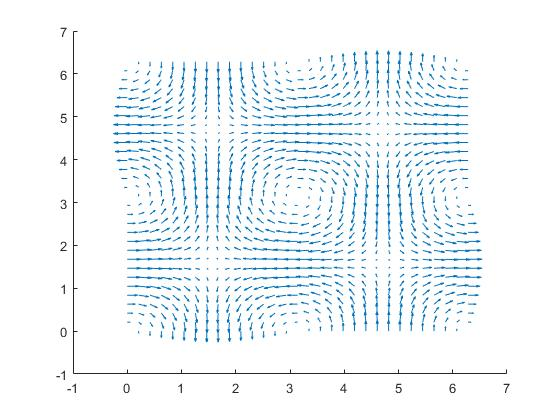
\includegraphics[width=\textwidth]{1b}

\subsection{c}
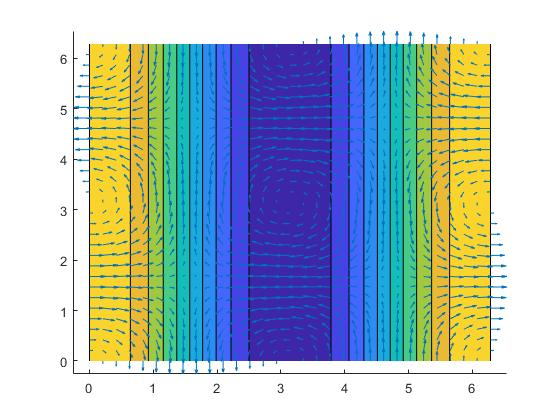
\includegraphics[width=\textwidth]{1c}

\subsection{d}
Attached video.

\subsection{e}
At a 101 points, the simulation becomes a lot finer and the resolution of the output increases. The model remains stable and does not shoot out to infinity. 

\subsection{f}
At a 501 points, the simulation slows down drastically as per the increased compuational cost. The model becomes unstable and values start shooting up/down to the infinities. The reason behind it is the stability condition given by: \newline
\newline



\section{Problem 2}
Attached video. \newline
\newline

Given the velocity profile is cyclic, assuming the discretization is perfect, the initial profile and final profile should look exactly the same. However, due to the approximation of the discretization function, the profile only approximately returns to the starting condition. Furthermore, if the time sampling increases or the number of points increases, the final profile better represents the expected value.

\end{document}

